\subsection{Vamos apresentar agora a letra B}

Agora vamos apresentar aqui o esquema em questão

Simulação do inciso B diagrama com a da amplitude  do degrau A=m/4=10/4=2.5

Logo aqui tem o diagrama do inciso B do diagrama com a Situação anterior vs a situação agora que tem o PID

Comentar sobre as situações


\begin{figure}[H]
    \centering
    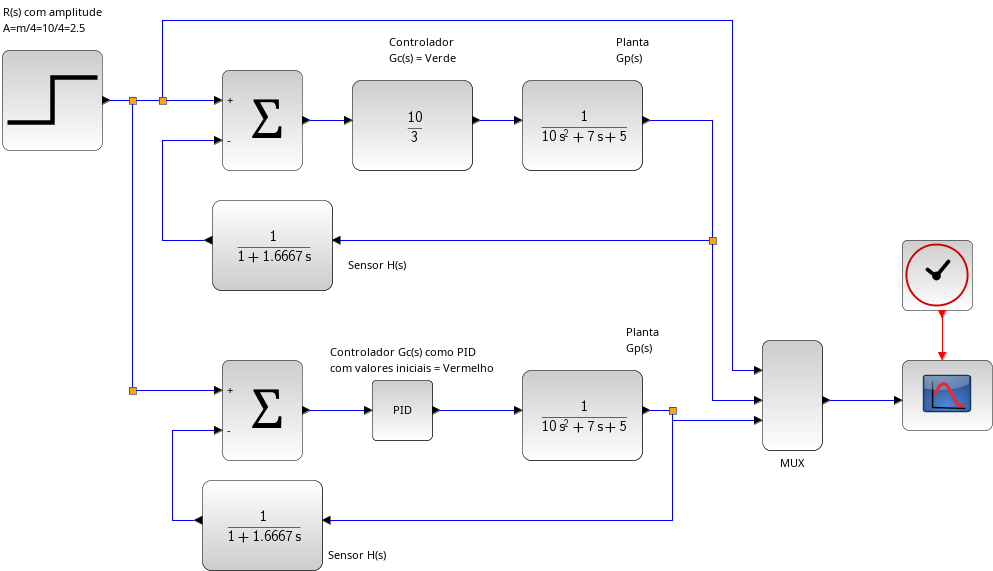
\includegraphics[width=0.8\textwidth]{6-atividade/assets/b/diagrama-comparacao-proporcional-pid.png}
    \caption{Resposta do sistema com os parâmetros do PID ajustados.}
    \label{fig:diagrama-comparacao-proporcional-pid}
\end{figure}

\begin{figure}[H]
    \centering
    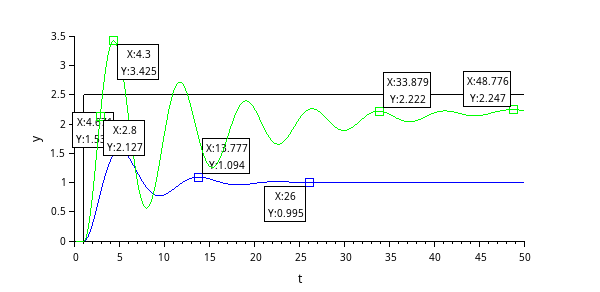
\includegraphics[width=0.8\textwidth]{6-atividade/assets/b/comparacao-proporcional-pid.png}
    \caption{Resposta do sistema com os parâmetros do PID ajustados.}
    \label{fig:comparacao-proporcional-pid}
\end{figure}

Onde a respsota azul é a resposta do sistema com controlador proporcional enquanto o verde é o controlador PID com os parametros referenciados anteriormente:
Os parâmetros \( K_p = 8.958 \), \( K_i = 0.310462589 \), e \( K_d = 0.80525 \) são implementados no controlador PID no ambiente de simulação,


ENtão comente e faça uma conclusão disso